\documentclass[aspectratio=169]{beamer}
%\usepackage[english,greek]{babel}
%\usepackage[iso-8859-7]{inputenc}
\usepackage{euler}
\usepackage{graphicx,pgfplots,tikz}

\beamertemplatenavigationsymbolsempty

\begin{document}
	\begin{frame}{$k=1$}
		\begin{figure}
			\resizebox{\linewidth}{!}{\begin{tikzpicture}
			\draw[thick,->] (-.5,0) -- (6,0);
			\draw[thick,->] (0,-.1) -- (0,3);
			\draw[blue, domain={0.01}:{5.8}, samples=100] plot (\x,{2*(\x+1)*exp(-\x)});
			\end{tikzpicture}}
		\end{figure}
	\end{frame}

\begin{frame}{$k=1.5$}
	\begin{figure}
		\resizebox{\linewidth}{!}{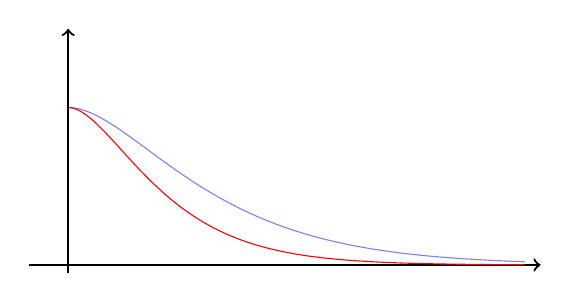
\begin{tikzpicture}
			\draw[thick,->] (-.5,0) -- (6,0);
			\draw[thick,->] (0,-.1) -- (0,3);
			\draw[blue, opacity=.5, domain={0.01}:{5.8}, samples=100] plot (\x,{2*(\x+1)*exp(-\x)});
			\draw[red, domain={0.01}:{5.8}, samples=100] plot (\x,{2*(1.5*\x+1)*exp(-1.5*\x)});
			\end{tikzpicture}}
	\end{figure}
\end{frame}

\begin{frame}{$k=2$}
	\begin{figure}
		\resizebox{\linewidth}{!}{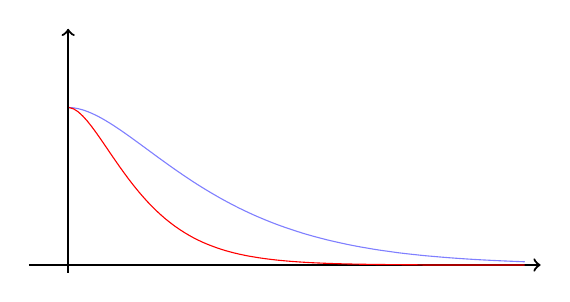
\begin{tikzpicture}
			\draw[thick,->] (-.5,0) -- (6,0);
			\draw[thick,->] (0,-.1) -- (0,3);
			\draw[blue, opacity=.5, domain={0.01}:{5.8}, samples=100] plot (\x,{2*(\x+1)*exp(-\x)});
			\draw[red, domain={0.01}:{5.8}, samples=100] plot (\x,{2*(2*\x+1)*exp(-2*\x)});
			\end{tikzpicture}}
	\end{figure}
\end{frame}

\begin{frame}{$k=2.5$}
	\begin{figure}
		\resizebox{\linewidth}{!}{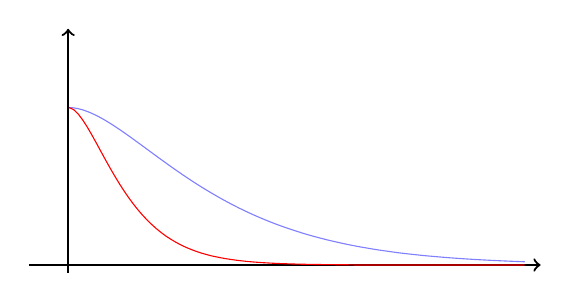
\begin{tikzpicture}
			\draw[thick,->] (-.5,0) -- (6,0);
			\draw[thick,->] (0,-.1) -- (0,3);
			\draw[blue, opacity=.5, domain={0.01}:{5.8}, samples=100] plot (\x,{2*(\x+1)*exp(-\x)});
			\draw[red, domain={0.01}:{5.8}, samples=100] plot (\x,{2*(2.5*\x+1)*exp(-2.5*\x)});
			\end{tikzpicture}}
	\end{figure}
\end{frame}

\begin{frame}{$k=3$}
	\begin{figure}
		\resizebox{\linewidth}{!}{\begin{tikzpicture}
			\draw[thick,->] (-.5,0) -- (6,0);
			\draw[thick,->] (0,-.1) -- (0,3);
			\draw[blue, opacity=.5, domain={0.01}:{5.8}, samples=100] plot (\x,{2*(\x+1)*exp(-\x)});
			\draw[red, domain={0.01}:{5.8}, samples=100] plot (\x,{2*(3*\x+1)*exp(-3*\x)});
			\end{tikzpicture}}
	\end{figure}
\end{frame}

\begin{frame}{$k=3.5$}
	\begin{figure}
		\resizebox{\linewidth}{!}{\begin{tikzpicture}
			\draw[thick,->] (-.5,0) -- (6,0);
			\draw[thick,->] (0,-.1) -- (0,3);
			\draw[blue, opacity=.5, domain={0.01}:{5.8}, samples=100] plot (\x,{2*(\x+1)*exp(-\x)});
			\draw[red, domain={0.01}:{5.8}, samples=100] plot (\x,{2*(3.5*\x+1)*exp(-3.5*\x)});
			\end{tikzpicture}}
	\end{figure}
\end{frame}

\begin{frame}{$k=4$}
	\begin{figure}
		\resizebox{\linewidth}{!}{\begin{tikzpicture}
			\draw[thick,->] (-.5,0) -- (6,0);
			\draw[thick,->] (0,-.1) -- (0,3);
			\draw[blue, opacity=.5, domain={0.01}:{5.8}, samples=100] plot (\x,{2*(\x+1)*exp(-\x)});
			\draw[red, domain={0.01}:{5.8}, samples=100] plot (\x,{2*(4*\x+1)*exp(-4*\x)});
			\end{tikzpicture}}
	\end{figure}
\end{frame}

\begin{frame}{$k=4.5$}
	\begin{figure}
		\resizebox{\linewidth}{!}{\begin{tikzpicture}
			\draw[thick,->] (-.5,0) -- (6,0);
			\draw[thick,->] (0,-.1) -- (0,3);
			\draw[blue, opacity=.5, domain={0.01}:{5.8}, samples=100] plot (\x,{2*(\x+1)*exp(-\x)});
			\draw[red, domain={0.01}:{5.8}, samples=100] plot (\x,{2*(4.5*\x+1)*exp(-4.5*\x)});
			\end{tikzpicture}}
	\end{figure}
\end{frame}

\begin{frame}{$k=5$}
	\begin{figure}
		\resizebox{\linewidth}{!}{\begin{tikzpicture}
			\draw[thick,->] (-.5,0) -- (6,0);
			\draw[thick,->] (0,-.1) -- (0,3);
			\draw[blue, opacity=.5, domain={0.01}:{5.8}, samples=100] plot (\x,{2*(\x+1)*exp(-\x)});
			\draw[red, domain={0.01}:{5.8}, samples=100] plot (\x,{2*(5*\x+1)*exp(-5*\x)});
			\end{tikzpicture}}
	\end{figure}
\end{frame}
\end{document}